%xelatex -shell-escape -output-directory=bin ergasia.tex
\documentclass{assignment}

\university{Πανεπιστήμιο Πειραιώς}{Πα.Πει.}
\school{Τμήμα Πληροφορικής}{Π.Μ.Σ. "Πληροφορική"}
\department{Πρόγραμμα Μεταπτυχιακών Σπουδών «Πληροφορική»}{}
%\cover{images/cover.jpg}{http://www.cyberciti.biz/faq/grub-boot-into-single-user-mode/}

\title{Τεχνολογίες Διαδικτύου \\ 2η Εργασία}
%\projectlevel{Εργαστήριο Λειτουργικά Συστήματα}
%\lesson{Λειτουργικά Συστήματα}{1}
\date{Αθήνα, 2014}

\author{Αναγνωστόπουλος Βασίλης - Θάνος, Κατσής Γεώργιος}
%\register{ΜΠΠΛ13002}{1}

%\exercauthor{Αναγνωστόπουλος Βασίλης - Θάνος}{06107083}{9}

%\advisor{Τσακίρη Μαρία, Αναπληρώτρια Καθηγήτρια Ε.Μ.Π.}

\begin{document}

\maketitle
% Να σκεφτώ τί αλλαγές θέλω να κάνω με τις αριθμήσεις και άμα θέλω να κάνω.
% Να σκεφτώ να τις ενσωματώσω και στο assignment.cls

\setcounter{page}{1} 
\pagenumbering{roman}

\pagestyle{plain}
\tableofcontents
\newpage


%\pagestyle{headings}
\pagestyle{fancy}
\setcounter{page}{1} 
\pagenumbering{arabic}

\begin{Assignment}%[Ερώτημα]
\AssignmentTitle{ % 
Δημιουργήστε μία ιστοσελίδα.

Παρατηρήσεις: Προσπαθήστε να μη χρησιμοποιήσετε περιττές ετικέτες HTML.
Η λέξη «Δίκτυα Υπολογιστών» είναι σύνδεσμος που οδηγεί στη διεύθυνση:
http://gunet2.cs.unipi.gr/eclass/courses/TME128/

Η λέξη «Κρυπτογραφία» είναι εσωτερικός σύνδεσμος που οδηγεί στο τμήμα της ιστοσελίδας με τιςαντίστοιχες πληροφορίες. 

Το λεκτικό Δουληγέρης Χρήστος είναι σύνδεσμος email που θα ανοίγει πρόγραμμα αποστολής ηλεκτρονικού ταχυδρομείου.

Προσέξτε ότι υπάρχουν μορφοποιήσεις (εκθέτες, έντονο, έμφασης κ.α ) σε διάφορες λέξεις τουκειμένου και το περιεχόμενο της ιστοσελίδας είναι (από πλευράς κώδικα) διαμορφωμένο σε τμήματα.

Ο χρήστης μπορεί να προσθέσει και άλλο μάθημα στη λίστα των μαθημάτων.

Το κείμενο μπορείτε να το αντλήσετε από τις ιστοσελίδες http://gunet2.cs.unipi.gr και http://www.cs.unipi.gr/

}

Ο κώδικας που υλοποιεί την σελίδα φαίνεται παρακάτω.

\inputminted[linenos,tabsize=2]{html}{../../index.html}
\captionof{listing}{Ο κώδικας της σελίδας \label{html_code}}


Ακόμα η σελίδα έχει "ανέβει" στην διεύθυνση \url{http://tme121.anagno.me}
και ο κώδικας της βρίσκεται στο \url{https://github.com/giokats/Texnologies_Diadiktiou}
\end{Assignment}

Τέλος ο κώδικας της σελίδας ελέγχθηκε χρησιμοποιώντας το \url{http://validator.w3.org} (εικόνα 
\ref{fig:date})

\begin{figure}
\begin{center}
\resizebox*{!}{8.5cm}{
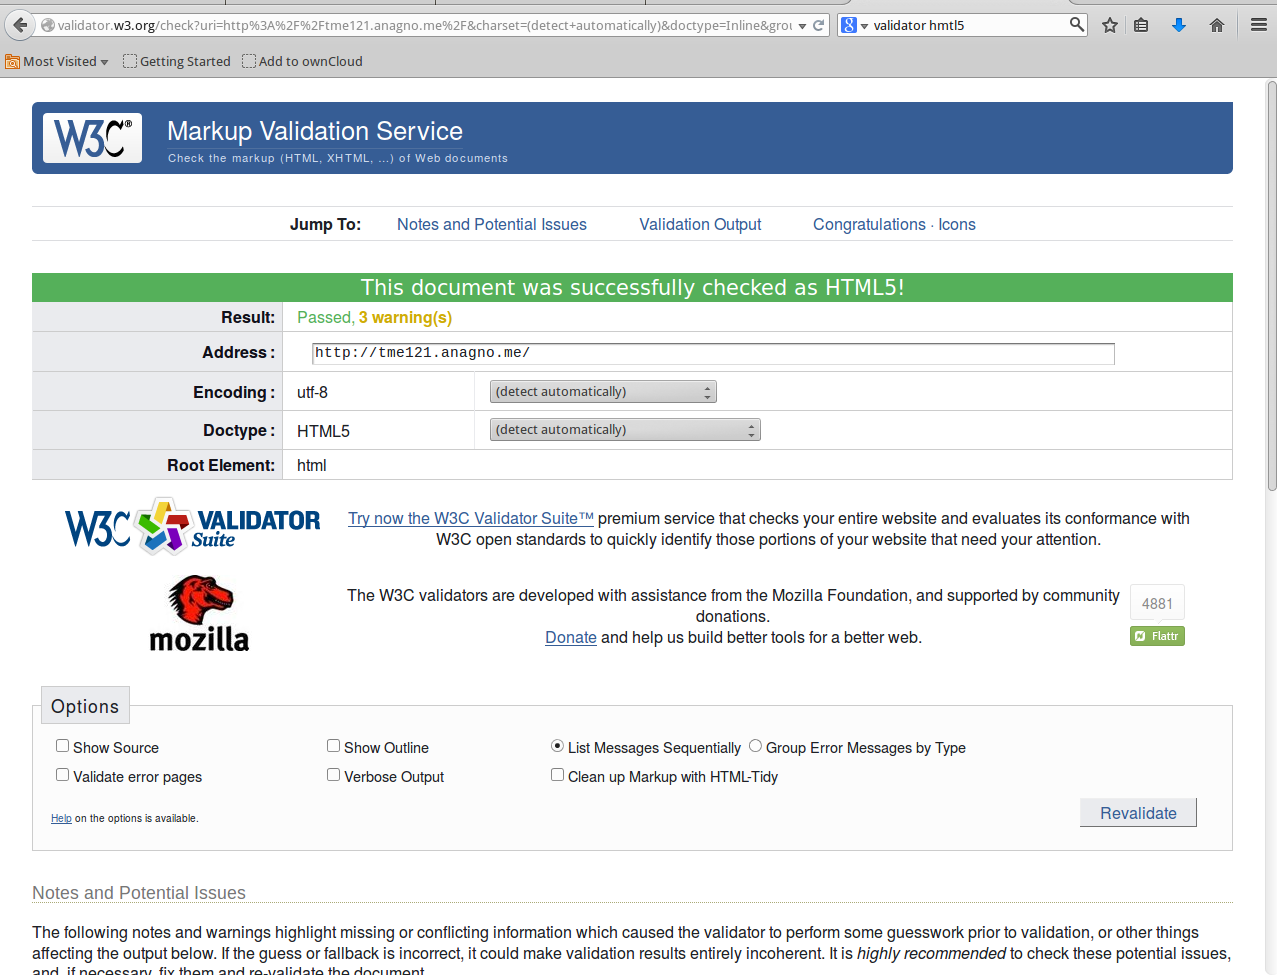
\includegraphics{images/validator.png}}
\caption{Screenshot από το \url{http://validator.w3.org} }
\label{fig:date}
\end{center}
\end{figure}

\begin{figure}
\begin{center}
\resizebox*{!}{8.5cm}{
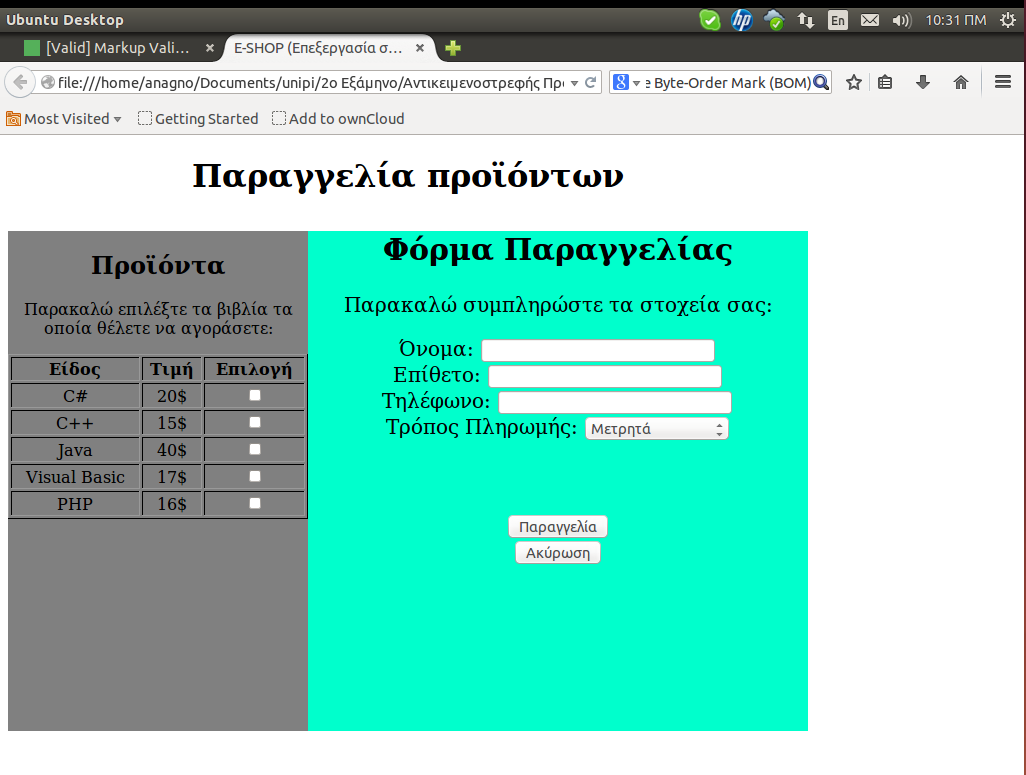
\includegraphics{images/site.png}}
\caption{Screenshot από την ιστοσελίδα χρησιμοποιώντας τον \en{firefox} }
\label{fig:site}
\end{center}
\end{figure}

\begin{figure}
\begin{center}
\resizebox*{!}{8.5cm}{
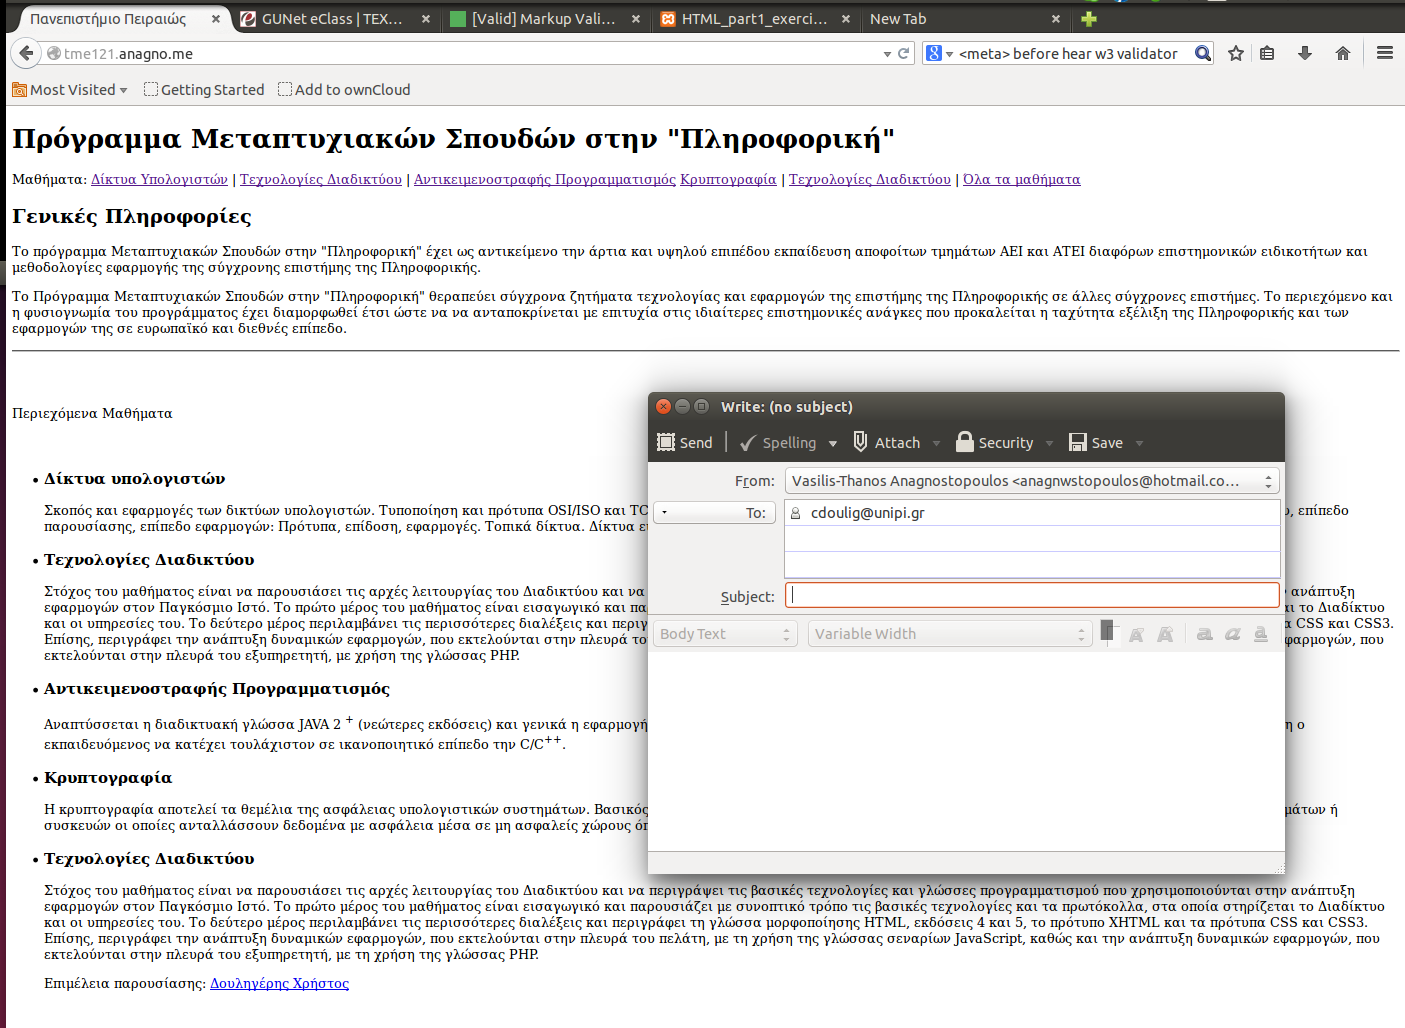
\includegraphics{images/mail.png}}
\caption{Screenshot έχοντας πατήσει το μαιλ χρησιμοποιώντας το \en{thunderbird} }
\label{fig:mail}
\end{center}
\end{figure}



\newpage

%\phantomsection \label{Βιβλιογραφία}
%\addcontentsline{toc}{section}{Βιβλιογραφία}
%\mtcaddchapter[Βιβλιογραφία] % Λόγω του minitoc
%\bibliographystyle{plain}
%\bibliography{references}


\end{document}

1
